\documentclass[12pt,a4paper]{report}

\usepackage[portuguese]{babel}
\usepackage{hyphenat}
\usepackage{amsmath}
\usepackage{amsfonts}
\usepackage{amssymb}
\usepackage{amsthm}
\usepackage{graphicx}
\usepackage{makeidx}

\usepackage[square,sort,comma,numbers]{natbib}
\usepackage[left=1in,right=1in,top=1in,bottom=1in]{geometry}
\usepackage{setspace}

\setstretch{1.5}

\hyphenpenalty
\exhyphenpenalty

\begin{document}

\begin{titlepage}
    {\centering
        {
        \LARGE{\textbf{Projeto Laboratórios de Informática III\\Fase 1}} \\ 
        \vspace*{\fill} 
        {\large{Projeto desenvolvido por}} \\
        \vspace{10pt}
        \small{ Fábio  Leite (A100902),  Luís Figueiredo (A100549) e Gonçalo Gonçalves (A100833) } \\
        \vspace{10pt}
        {\large{Grupo 50}}
        \vspace*{\fill} \\
        {\Large Licenciatura em Engenharia Informática} \\
        \vspace*{\fill}
        
\includegraphics[scale=1.25]{eeng.png} \\ [0.5cm]
        {\large Departamento de Informática \\ Universidade do Minho} \\
        }
    }
\end{titlepage}

\newpage

    \tableofcontents

\newpage

    \chapter{Introdução}
        
        \paragraph{} Este projeto foi desenvolvido no âmbito da unidade curricular de Laboratórios de Informática III do ano 2023/2024. Neste projeto, fomos instruídos a implementar uma base de dados em memória que armazene dados fornecidos em arquivos ".csv".
        \par Após a conclusão da primeira fase, começamos por fazer melhorias em relação as \textit{queries} anteriormente feitas, deixando de iterar \textit{hash tables}, recolhendo grande parte dos dados necessários através do \textit{parsing} dos dados. Melhorámos também um dos nossos pontos mais fracos na primeira fase, a validação, que agora se encontra finalmente completa.
        Após isso, tratamos também da implementação do modo interativo, que nos permite interagir com o programa através do terminal, não funcionando através do fornecimento do input na forma de um ficheiro.
        Nesta fase também foi criado um programa de testes, que permite-nos comparar localmente os outputs criados pelo nosso programa com os outputs supostos.
        
    \chapter{Arquitetura e estrutura}
    \par Recapitulando a arquitetura apresentada na primeira fase, o armazenamento de dados foi feito em 3 \textit{hash tables} para os ficheiros que apresentavam mais dados, neste caso, os \textit{users}, \textit{flights} e \textit{reservations}, e uma \textit{GList} para os \textit{passengers}. Cada linha de cada ficheiro ".csv" seria guardado numa \textit{struct} que representa a respetiva entidade (\textit{user}, \textit{flight}, \textit{passenger} ou \textit{reservation}) e cada ficheiro seria guardado num catálogo. Após isso, seria feito o \textit{parsing} e a validação de cada linha de modo a garantir que só as entradas válidas seriam guardadas nos catálogos e as entradas inválidas seriam escritas no ficheiro de erros. Já com os catálogos devidamente preenchidos, o \textit{interpreter} é chamado para a realização das \textit{queries} e a geração dos ficheiros é feito pelo módulo output.
    \par Face à avaliação feita na primeira fase, decidimos seguir o conselho na implementação de um módulo chamado Stats de modo a suavizar a execução das \textit{queries}. Neste módulo, foram implementadas estruturas auxiliares onde serão guardados os dados necessários para a realização das várias \textit{queries}, aquando do \textit{parsing} e da validação dos ficheiros. Todo este trabalho adicional realizado no \textit{parsing} e na validação traz ganhos significativos aquando da realização das \textit{queries}, embora cause um aumento de tempo no \textit{startup} do programa.
    \par No módulo Stats implementámos 3 estruturas auxiliares: hotel, airportS e dictionary. Na estrutura hotel, é mantida a lista de reservas de um hotel, assim como o número de reservas e o somatório das avaliações desse mesmo hotel e o {id} do hotel. Na estrutura airportS, são mantidas o nome do aeroporto(origin),uma lista de atrasos dos voos que partem desse mesmo aeroporto,a mediana desses atrasos e uma lista que contém os \textit{flights} que partem do aeroporto em questão. 
\newpage

Na figura abaixo (Figura 2.1) apresentamos um diagrama que sintetiza o funcionamento do nosso programa em condições normais (modo Batch).

    \begin{figure}[h]
    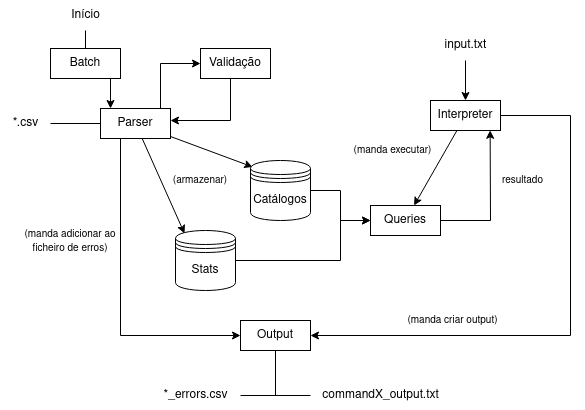
\includegraphics[scale = 0.6]{Batch.png}
    \centering
    \caption{Diagrama do funcionamento do modo Batch}
    \end{figure} 

    
    \chapter{Queries}
    Tivemos alguns problemas na implementação de certas \textit{queries}, especialmente na \textit{query} 9 aonde a mesma corre normalmente localmente, enquanto a mesma produz \textit{segmentation fault} no site de testes.
    Nesta fase conseguimos implementar 5 \textit{queries} corretamente e apresentamos 2 que estão a falhar em casos específicos.
    
    \textbf{Query 1:}
    \par Nesta \textit{query} é nos fornecido o {id} de uma entidade do sistema, e através dela temos de listar certas informações que são pedidas. Grande parte desta \textit{query} é baseada na obtenção de dados através dos catálogos. Informações como o total gasto por um utilizador ou o seu número de reservas são obtidas durante o \textit{parsing} e guardadas em conjunto com a entidade específica.

    \textbf{Query 2:}

     \par Nesta \textit{query} o objetivo era listar os voos ou reservas de um utilizador, se o segundo argumento for \textit{flights} ou \textit{reservations}, respetivamente, ordenados por data de inicio, e caso não fosse dado um segundo argumento, listar as \textit{reservations} e os \textit{flights} em conjunto.
     \par Para a realização desta \textit{query} foram usados dados obtidos no Parser e guardados em conjunto com o \textit{user}, sendo eles duas listas compostas pelos voos e pelas reservas feitas por um utilizador.
\newpage
     \par \textbf{Query 3:}
     \par O objetivo desta \textit{query}  era apresentar a classificação média de um hotel, a partir do seu identificador.
        Para a resolução desta \textit{query} utilizamos uma \textit{hash table} composta por objetos do tipo \textbf{HOTEL*} criados no ficheiro das estatísticas. Estes objetos são compostos por informações necessárias para o desenvolvimento de uma \textit{query} que envolva um hotel. Para esta \textit{query} é utilizada a soma do \textit{rating} do hotel e o número de reservas feitas no mesmo para calcular o \textit{rating} médio, sendo estes dados obtidos quando é feito o Parser.


    \textbf{Query 4:}
     \par  O objetivo desta \textit{query} era listar as reservas de um hotel, ordenadas por data de início.
        Para esta \textit{query} foi utilizada a mesma estrutura  "hotel", aonde se vai buscar uma lista (\textit{GList}) que apresenta todas as reservas feitas no hotel especificado no argumento dado à função.

     \textbf{Query 5:}
     \par Esta \textit{query} tinha como objetivo listar os voos com origem num dado aeroporto, entre duas datas.Para a resolução desta \textit{query} criamos no ficheiro das estatísticas uma \textit{hash table} composta por objetos do tipo \textbf{AIPORTS*}.
     Após recolhermos o aeroporto especificado no input,vamos a esse objeto buscar a lista de voos que partem do mesmo (lista obtida durante o \textit{parsing} dos dados), ordenando-a com a ajuda de funções da GLib.

     \textbf{Query 6:}
     \par Esta \textit{query} tinha como objetivo listar o top N aeroportos com mais passageiros, para um dado ano. Para \textit{query} utilizamos a mesma estrutura "airportS", aonde vamos buscar a cada voo ,presente na lista de voos que partem de um dado aeroporto,  o número de passageiros e o aeroporto de onde parte e o aeroporto para onde se dirige. Através desses dados,criamos uma nova \textit{hash table} que armazena o número de passageiros de cada aeroporto.

     \textbf{Query 7:}
    \par Relativamente à \textit{query} 7, o objetivo da mesma era listar o top N aeroportos com a maior mediana de atrasos.
    Utilizando novamente a estrutura dos aeroportos, cada vez que foi executado o \textit{parsing} de um voo foi guardado numa lista o atraso correspondente ao mesmo, sendo essa lista pertencente ao aeroporto de onde o voo partia.
    \par Através desta lista foi calculada a mediana de atrasos de cada aeroporto, de forma a ser possível ordenar os aeroportos.
    
    
    \chapter{Modo interativo}
    \par Quando se executa o programa no modo Interativo, este é o comportamento do programa:    
    
    \begin{figure}[h]
    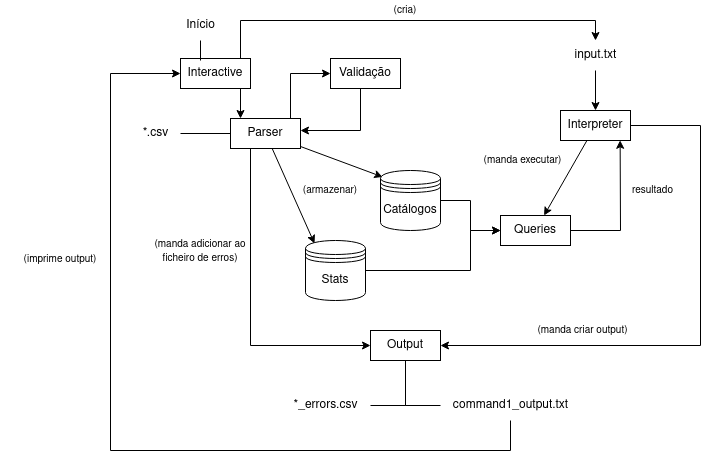
\includegraphics[scale = 0.6]{Interactive.png}
    \centering
    \caption{Diagrama do funcionamento do modo Interativo}
    \end{figure} 

    \par Como podemos ver nesta figura, o módulo Interactive substitui o Batch. A principal diferença é que o Interactive cria um \textit{loop} imprimindo um sistema de menus e, dependendo do que o utilizador escolher, cria um ficheiro chamado input.txt com a \textit{query} e as informações desejadas, chegando assim a um estado em que o programa se comporta como se estivesse a correr em modo Batch com apenas uma \textit{query} no input.txt e, posteriormente, o Interactive lê o ficheiro de output criado e imprime o output na terminal, voltando assim ao sistema de menus (o programa só termina caso o utilizador selecione a respetiva opção no menu ou caso seja interrompido). Apesar de não ser a forma ideal de implementar este modo em termos de eficiência, foi feito assim de modo a garantir uma substituição direta do módulo Batch pelo Interactive, o que leva à reutilização da totalidade do restante código desenvolvido, que é um dos focos principais desta fase de desenvolvimento. 

    
    \chapter{Programa-testes}

    Quando se executa o programa-testes, este é o comportamento do programa:    
    
    \begin{figure}[h]
    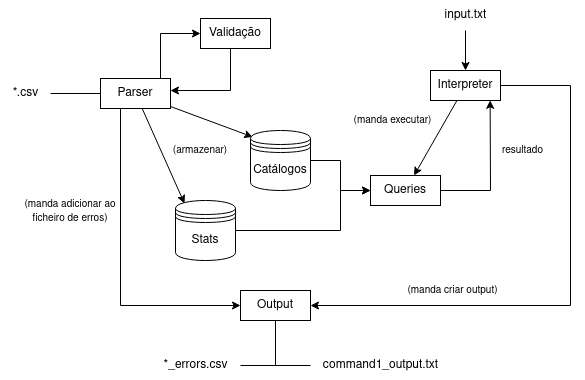
\includegraphics[scale = 0.6]{Testes.png}
    \centering
    \caption{Diagrama do funcionamento do programa-testes}
    \end{figure} 

     A estrutura é semelhante ao programa da primeira fase (com a adição do Stats) uma vez que considerámos que não faz sentido existir aqui um modo interativo. Isto leva à reutilização de praticamente todos os módulos do programa (excluindo o Interativo), o que é um dos focos principais do projeto.

    Depois do programa "principal" correr, são comparados todos os resultados obtidos com os resultados esperados (passados como argumento) linha a linha para ver se existe alguma incongruência, se existir, o programa imprime o comando e a linha onde esta ocorre e no fim é imprimido o número do comando onde a primeira incongruência foi encontrada caso esta exista ou, no caso de não existir, é imprimida a mensagem "Todos os testes passaram!". Foi optado por ignorar os ficheiros de \textit{output} que não foram criados de modo a não haver demasiada informação imprimida na terminal, uma vez que não foram implementadas todas as \textit{queries}.
    
    O programa mede e imprime o tempo de execução geral do programa e faz o mesmo para cada \textit{query} individualmente. O tempo de execução geral do programa é calculado antes de comparar os resultados de modo a garantir um tempo de execução mais próximo do real (quando se usa o modo Batch no Programa-principal). Para além disto o programa também calcula a memória máxima usada.

    
    \chapter{Desempenho}

     Para testar o desempenho final do programa foi utilizado o programa-testes para saber o tempo total de execução e a memória máxima utilizada. Como não conseguimos adaptar o programa para usar o \textit{dataset} grande, foi utilizado o \textit{dataset} com entradas inválidas da 1ª fase com um \textit{input} de 100 \textit{queries}. Os tempos finais foram obtidos ao executar o programa 20 vezes em cada máquina e calculando a média dos tempos de cada execução.

    \par Estes são os resultados da execução nas 3 máquinas pertencentes aos elementos do grupo:
    
\begin{table}[htbp]
    \begin{center}
    \begin{tabular}{|p{3cm}|p{4cm}|p{4cm}|p{4cm}|}
    \hline
                                           & \textbf{Máquina 1} &                        \textbf{Máquina 2} &                       \textbf{Máquina 3} \\ \hline
    \textbf{CPU}            & Intel Core i7-8550U  @ 1.80GHz            & Intel Core i7-10750H @ 2.60GHz                 & Intel Core i7-10750H @ 2.60GHz\\ \hline
    \textbf{Cores/Threads}                    & 4/8                                          & 6/12                                  & 6/12\\ \hline
    \textbf{RAM}                              & 8 GB DDR4                                    & 10 GB DDR4 2933                       & 16GB DDR4\\ \hline
    \textbf{Disco}                            & 256 GB SSD                                   & 512 GB SSD                            & 1 TB SSD\\ \hline
    \textbf{OS}                               & Ubuntu 22.04.3 LTS                           & Ubuntu 22.04.3 LTS (VM)                    & Ubuntu 20.04.6 LTS\\ \hline
    \textbf{Compilador/ Versão}               & gcc 11.4.0                                   & gcc 11.4.0                     & gcc 9.4.0 \\ \hline
    \textbf{Pico de memória}                  & 44800 KB                                     & 44928 KB                              & 43728 KB\\ \hline
    \textbf{Tempo geral de execução}      & 0,634 s                                   & 0,521 s                            & 0.311 s\\ \hline
    \textbf{Tempo de execução do \textit{parser}} & 0.531 s                            & 0.453 s                                  & 0.253 s \\ \hline
    \textbf{Percentagem de tempo no \textit{parser}} & 83.75\%                          & 86.94\%                                 &  81,35\%        \\ \hline
    \end{tabular}
    \end{center}
    \caption{tabela de desempenho}
    \label{tab:exemplo2}
\end{table}

    Estes resultados proporcionam uma visão geral do desempenho relativo das três máquinas. A máquina 3 destacou-se com o melhor desempenho global, seguida pela máquina 2 que tem o 2º menor tempo mas tem o pico de memória mais alto e, por último, a máquina 1 que tem o pior tempo mas tem o 2º pico de memória mais baixo.

    Com base nos resultados obtidos, acredita-se que o desempenho das \textit{queries} tenha sido eficiente devido à utilização de estruturas de dados adequadas. A adoção de três tabelas \textit{hash tables} e uma \textit{GList} demonstrou-se eficaz na organização e manipulação dos dados, contribuindo assim para a rapidez e eficiência das consultas.

    Como o tempo de \textit{parsing} dos dados é cerca de 80\% do tempo de execução geral, identificamos que este é elo mais fraco em termos de execução. O facto desta etapa ser particularmente lenta é a principal limitação que restringe a capacidade de realizar testes em larga escala, o que leva ao nosso \textit{timeout} quando é testado o \textit{dataset} grande.

    Em suma, apesar dos desafios identificados, estamos confiantes na solidez das estruturas de dados adotadas e no potencial de otimização do sistema mas, infelizmente, não fomos capazes de otimizar o programa como queríamos a tempo da entrega do projeto.  



    \chapter{Dificuldades sentidas}
    \paragraph{} Ao longo do desenvolvimento do projeto, fomos encontrando diversos problemas que, para além de produzirem resultados errados, também impediram o nosso progresso.
    A maior dificuldade sentida nesta fase foi a tentativa de colocar o nosso programa a correr os testes de maiores dimensões, uma vez que o tempo de execução dos mesmos supera o limite estabelecido pela plataforma de testes.
    \par Da mesma forma, certas \textit{queries} levantaram-nos dúvidas, especialmente a \textit{query} 9. Nesta \textit{query}, a nossa dúvida principal é provocada pelo facto de a mesma provocar \textit{segmentation fault} na plataforma de testes, embora a mesma não o faça localmente. Este erro já existiu na primeira fase de avaliação, e mesmo após uma reestruturação da mesma, continua a provocar problemas na execução do programa.
    \par Por fim, a utilização da \textit{glib}, embora traga bastantes benefícios,também traz uma maior complexidade para o projeto, sendo necessários vários momentos de pesquisa e teste para perceber as funcionalidades que as estruturas de dados e as funções desta mesma biblioteca apresentam. Um dos erros principais provados pela biblioteca foi a utilização de estruturas de dados, onde certas listas iniciavam em pontos diferentes cada vez que era dado um input à \textit{query} (erro ocorrido na \textit{query} 5). Aconteceu também de não conseguirmos atingir a execução sem \textit{memory leaks} devido a duas ocorrências estranhas relacionadas com \textit{GLists} que gostaríamos de discutir na apresentação com os professores, uma vez que gastámos muitas horas a tentar resolvê-las, mas sem sucesso.

    
    \chapter{Conclusão}
    \par Apesar de não termos conseguido implementar os requisitos na totalidade, considerámos que foi feito um bom trabalho, uma vez que esta segunda fase foi um grande desafio, com muitos conceitos novos e de implementação complexa.
    \par Para esta fase também apresentamos uma organização melhorada do código, tornando-o melhor estruturado e mais legível do que na fase anterior.
    \par Sentimos que melhoramos o nosso trabalho em relação à fase anterior em todos os aspetos, e que aplicamos corretamente os fundamentos base deste projeto, como a modularidade e encapsulamento, que pensamos serem conceitos fundamentais para o bom funcionamento do programa.





\end{document}
